% Generated by support/export-artifacts.py; do not edit.
% Slug: ch52-lifetime
% Source: chapters/ch52.tex:193
% TikZ source: chapters/ch52.tex:195
% Original label: \label{fig:ch52-lifetime}
% Original caption (LaTeX source):
%   Synchronous continuation calls preserve candidate lifetimes through commitment; no candidate pointer escapes the search stack.
% Caption: Synchronous continuation calls preserve candidate lifetimes through commitment; no candidate pointer escapes the search stack.
% Setup: support/compiler-pseudocode.sty (TikZ libraries and shared styles).
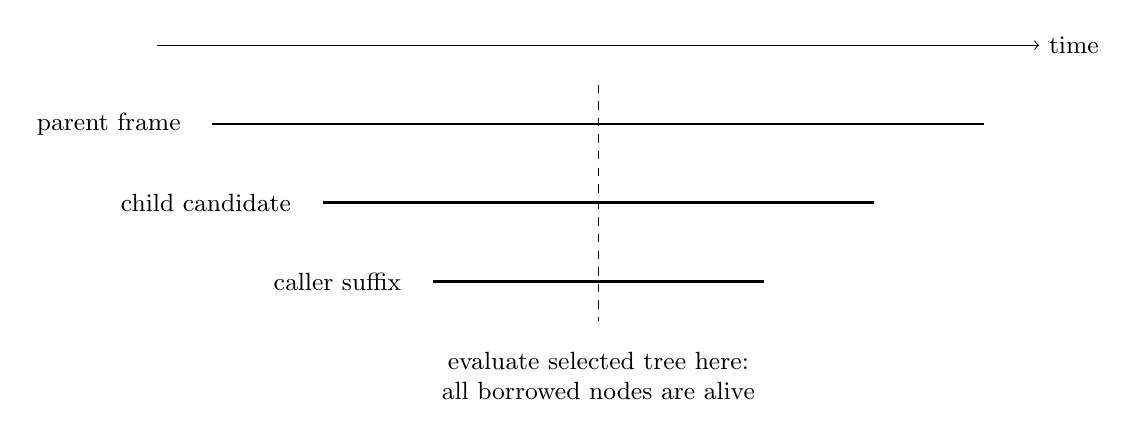
\begin{tikzpicture}[x=14mm,y=10mm]
\draw[->] (0,0)--(8,0) node[right,font=\small] {time};
\draw[line width=1pt] (0.5,-1)--(7.5,-1);
\draw[line width=1pt] (1.5,-2)--(6.5,-2);
\draw[line width=1pt] (2.5,-3)--(5.5,-3);
\draw[dashed] (4,-0.5)--(4,-3.5);
\node[anchor=east,font=\small] at (0.3,-1) {parent frame};
\node[anchor=east,font=\small] at (1.3,-2) {child candidate};
\node[anchor=east,font=\small] at (2.3,-3) {caller suffix};
\node[font=\small,align=center] at (4,-4.2) {evaluate selected tree here:\\all borrowed nodes are alive};
\end{tikzpicture}

% Original figure LaTeX:
% \begin{figure}[htbp]
% \centering
% \begin{tikzpicture}[x=14mm,y=10mm]
% \draw[->] (0,0)--(8,0) node[right,font=\small] {time};
% \draw[line width=1pt] (0.5,-1)--(7.5,-1);
% \draw[line width=1pt] (1.5,-2)--(6.5,-2);
% \draw[line width=1pt] (2.5,-3)--(5.5,-3);
% \draw[dashed] (4,-0.5)--(4,-3.5);
% \node[anchor=east,font=\small] at (0.3,-1) {parent frame};
% \node[anchor=east,font=\small] at (1.3,-2) {child candidate};
% \node[anchor=east,font=\small] at (2.3,-3) {caller suffix};
% \node[font=\small,align=center] at (4,-4.2) {evaluate selected tree here:\\all borrowed nodes are alive};
% \end{tikzpicture}
% \caption{Synchronous continuation calls preserve candidate lifetimes through commitment; no candidate pointer escapes the search stack.}
% \label{fig:ch52-lifetime}
% \end{figure}
